\documentclass{article}
\usepackage{pgfplots}
\pgfplotsset{
    compat=1.18,
    width=10cm,
    }

\begin{document}
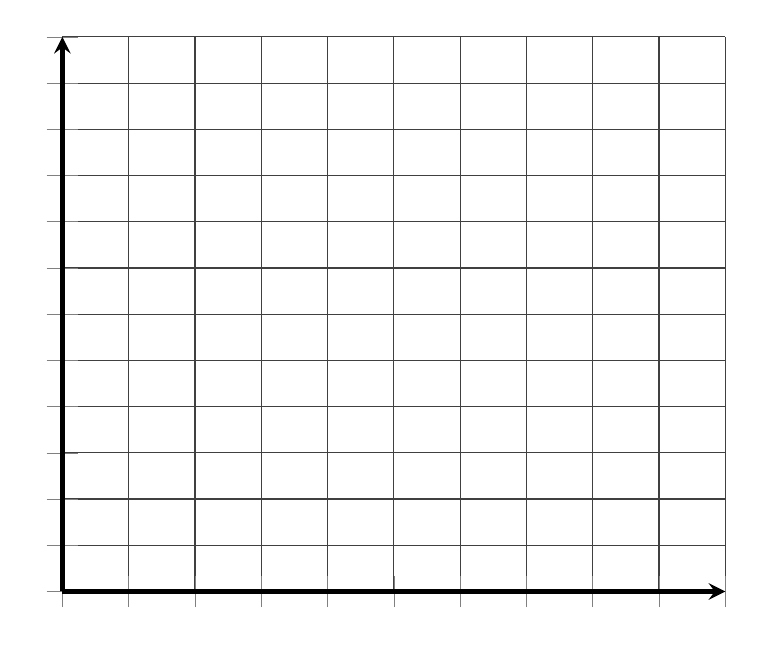
\begin{tikzpicture}
    \begin{axis}[
        xmin=0, xmax=10,
        ymin=0, ymax=60,
        axis lines=left,
        axis line style={ultra thick},
        xtick distance=1,
        ytick distance=5,
        xticklabels=\empty,
        yticklabels=\empty,
        major tick length={0.4cm},
        grid=both,
        grid style={solid,darkgray},
        ]
        \addplot[
            color=red,
            style=ultra thick,
            draw=none,
        ] coordinates {
            (0,0)(2.5,20)(4,20)(4.25,5)
        };
    \end{axis}
\end{tikzpicture}

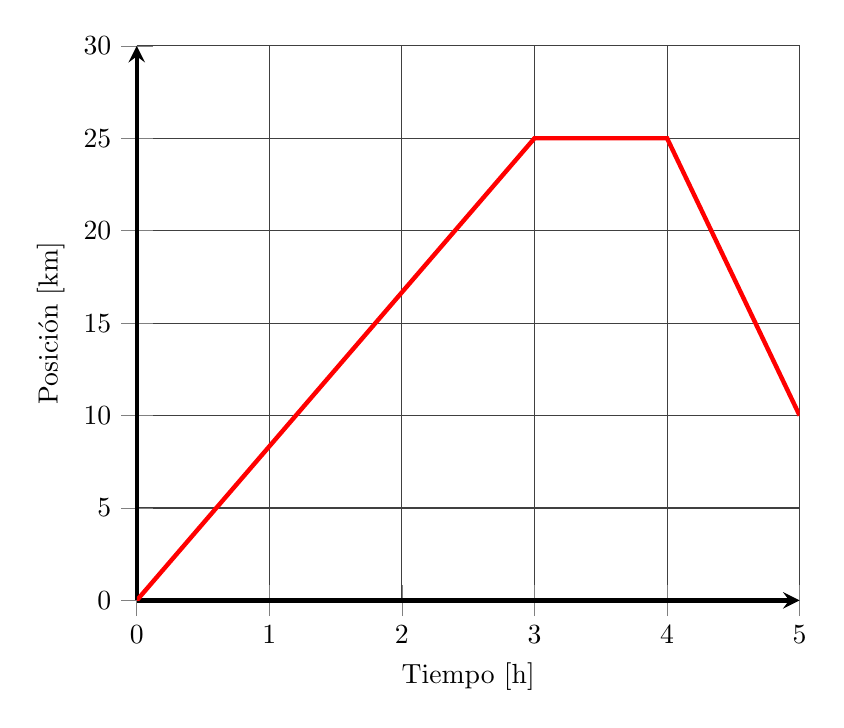
\begin{tikzpicture}
    \begin{axis}[
        xlabel={Tiempo [h]},
        ylabel={Posición [km]},
        xmin=0, xmax=5,
        ymin=0, ymax=30,
        axis lines=left,
        axis line style={ultra thick},
        xtick distance=1,
        ytick distance=5,
        major tick length={0.4cm},
        grid=both,
        grid style={solid,darkgray},
        ]
        \addplot[
            color=red,
            style=ultra thick,
        ] coordinates {
            (0,0)(3,25)(4,25)(5,10)
        };
    \end{axis}
\end{tikzpicture}
\end{document}